\documentclass[alsotrans]{beamerswitch}
\usepackage{sdp}

\title{Опашка}

\date{21--28 октомври 2019 г.}

\titlegraphicx{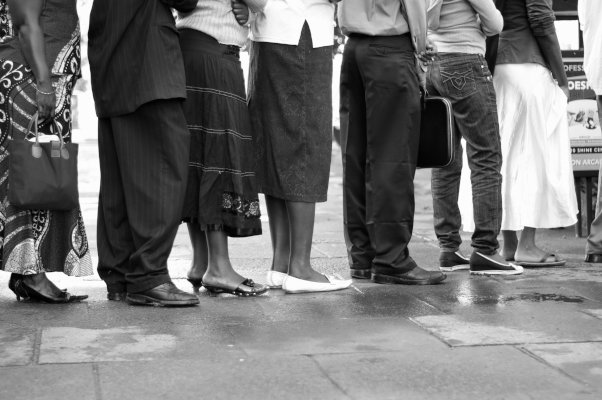
\includegraphics[height=0.25\textheight]{images/queue.jpg}\\
  \imageAttr{Queue}{Xiaojun Deng}{https://flic.kr/p/7sY2kp}{CC BY 2.0}}

% декорация за метода на вълната
\usetikzlibrary{decorations.pathmorphing}

\begin{document}

\begin{frame}
  \titlepage
\end{frame}

\section{АТД опашка}

\begin{frame}
  \frametitle{АТД: опашка}

  Хомогенна линейна структура с организация ``пръв влязъл --- пръв излязъл'' (FIFO)\\[1em]
  Операции:\\[0.5em]
  \begin{itemize}
  \item \lst{create()} --- създаване на празна опашка
  \item \lst{empty()} --- проверка за празнота на опашка
  \item \lst{enqueue(x)} --- включване на елемент в края на опашката
  \item \lst{dequeue()} --- изключване на елемент от началото на опашката
  \item \lst{head()} --- достъп до първия елемент
  \end{itemize}
\end{frame}

\begin{frame}
  \frametitle{АТД: опашка}

  Свойства на операциите\\[0.5em]
  \small
  \begin{itemize}
  \item \lst{create().empty()} = \lst{true}
  \item \lst{q.enqueue(x).empty()} = \lst{false}
  \item \lst{create().head()}, \lst{create().dequeue()} --- \alert{грешка}
  \item \tt{create().enqueue(x$_1$).enqueue(x$_2$)\ldots{}enqueue(x$_n$).head() = x$_1$}
  \item \tt{create().enqueue(x$_1$).enqueue(x$_2$)\ldots{}enqueue(x$_n$).dequeue() = create().enqueue(x$_2$)\ldots{}enqueue(x$_n$)}
  \end{itemize}
\end{frame}

\begin{frame}<1-| trans:1>
  \frametitle{Последователно представяне}

  \begin{center}
    \begin{tikzpicture}
      % масивът
      \matrix (a) [widearray] {
        |(an+5)| \only<all:7>{a_{n+5}} \&\&
        |(a0)| a_0 \& |(a1)| a_1 \& a_2 \& \ldots \& |(an)| a_n \&
        |(an+1)| \only<all:3->{a_{n+1}} \&
        |(an+2)| \only<all:4->{a_{n+2}} \&
        |(an+3)| \only<all:5->{a_{n+3}} \&
        |(an+4)| \only<all:6->{a_{n+4}} \\
      };

      % индекс на началото на опашката
      \pointerto[visible on=<all:1>]{a0}{\tt{front}}{below}

      % индекс на началото на опашката след премахване на елемент
      \pointerto[visible on=<all:2->]{a1}{\tt{front}}{below}

      % индекс на края на опашката
      \pointerto[visible on=<all:1-2>]{an}{\tt{back}}{below}

      % последователно добавяне на пет елемента
      \foreach \i in {1, ..., 5}{
        \tikzmath {
          int \j;
          \j = 2 + \i;
        }
        \pointerto[visible on=<all:\j>]{an+\i}{\tt{back}}{below}
      };
    \end{tikzpicture}
  \end{center}
  \begin{itemize}
    \item<2-> изключване на елемент (dequeue)
    \item<3-> включване на елемент (enqueue)
  \end{itemize}
\end{frame}

\begin{frame}<1-8| trans:1>
  \frametitle{Свързано представяне}

  \begin{center}
    \scriptsize
    \begin{overlayarea}{\textwidth}{.4\textheight}
      \begin{tikzpicture}
        % веригата
        \doublecell[visible on=<all:1-7>]{a0}{a_0}
        \doublecell[right=2em of a0next]{a1}{a_1}
        \draw[pointer,visible on=<all:1-7>] (a0next.center) to (a1data);

        \node (dots) [right=1em of a1] {...\hspace{1em}};
        \draw[pointer] (a1next.center) to (dots.west);

        \doublecell[right=1em of dots]{an-1}{a_{n-1}}
        \draw[pointer] (dots.east) to (an-1data);

        \nextdoublecell{an}{a_n}{an-1}
        \nullptr[visible on=<all:1-2>]{annext}

        % указател към началото
        \pointerto[visible on=<all:1-5>]{a0.south}{\tt{front}}{below}

        % указател към края
        \pointerto[visible on=<all:1-3>]{an.south}{\tt{back}}{below}

        % създаване на нова клетка, сочеща към null
        \begin{scope}[visible on=<all:2->]
          \doublecell[right=2em of annext]{an+1}{a_{n+1}}
          \nullptr{an+1next}
        \end{scope}

        % първоначално се сочи от указател p, а после от back
        \pointerto[visible on=<all:2->]{an+1.south}{\tt{\alt<all:2-3>p{back}}}{below}

        % указателят на предишната последна клетка се насочва към новата последна
        \draw[pointer,visible on=<all:3->] (annext.center) to (an+1data);

        % нов указател към първата клетка
        \pointerto[visible on=<all:5-7>]{a0}{\tt{p}}{above}

        % указателят front се насочва към втората клетка
        \pointerto[visible on=<all:6->]{a1}{\tt{front}}{below}

        % изтриване на първата клетка
        \draw (a0) node[cross,visible on=<all:7>] {};
      \end{tikzpicture}
    \end{overlayarea}
  \end{center}
  \begin{itemize}
    \item<2-> включване на елемент (enqueue)
    \item<5-> изключване на елемент (dequeue)
  \end{itemize}
\end{frame}

\section{Задачи}

\begin{frame}
  \frametitle{Числа на Hamming}

  \begin{definition}
    Казваме, че $k$ е число на Hamming, ако простите делители на $k$ са сред 2, 3 и 5, т.е. $k = 2^x3^y5^z$ за $x,y,z\geq 0$.
  \end{definition}

  \textbf{Задача.} Да се изведат в нарастващ ред първите $n$ числа на Hamming.\\
  \pause
  \textbf{Решение:}
  \begin{center}
    \begin{tikzpicture}[hmtx/.style={mtx,nodes={minimum width=2em}}]
      \matrix[hmtx,label=left:$q_2$] (q2) {
        \only<3-4>{\alert<4>2}\&\only<4-6>{\alert<6>4}\&\only<5-8>{\alert<8>6}\&\only<6->8\&\only<7->{10}\&\only<8->{12}\&\&\&\&\&\\
      };
      \matrix[hmtx,label=left:$q_3$,below=1ex of q2] (q3) {
        \only<3-5>{\alert<5>3}\&\only<4-8>{\alert<8>6}\&\only<5->9\&\only<6->{12}\&\only<7->{15}\&\only<8->{18}\&\&\&\&\&\\
      };
      \matrix[hmtx,label=left:$q_5$,below=1ex of q3] (q5) {
        \only<3-7>{\alert<7>5}\&\only<4->{10}\&\only<5->{15}\&\only<6->{20}\&\only<7->{25}\&\only<8->{30}\&\&\&\&\&\\
      };
    \end{tikzpicture}\\[1em]
    1%
    \onslide<5->{, 2}%
    \onslide<6->{, 3}%
    \onslide<7->{, 4}%
    \onslide<8->{, 5}%
    \onslide<9->{, 6, \ldots}
  \end{center}
\end{frame}

\begin{frame}
  \frametitle{Числа на Hamming: коректност}

  Да се докаже, че:
  \begin{enumerate}[<+->]
  \item се извеждат \textbf{всички} числа на Hamming\\
    \begin{proof}<+->
       Индукция: $2^x3^y5^z$ се извежда, понеже $2^{x-1}3^y5^z$ се извежда.
    \end{proof}
  \item се извеждат \textbf{само} числа на Hamming\\
    \begin{proof}<+->
      Ако извадим $2^x3^y5^z$, в опашките се записват $2^{x+1}3^y5^z$, $2^x3^{y+1}5^z$, $2^x3^y5^{z+1}$.
    \end{proof}
  \item числата на Hamming се извеждат във възходящ ред\\
    \begin{proof}<+->
      Да допуснем, че на края на някоя опашка добавяме по-малко число. Тогава на предна стъпка трябва да сме добавили по-малко число!
    \end{proof}
  \end{enumerate}
\end{frame}

\begin{frame}<1-9>
  \frametitle{Минимален елемент на опашка}

  \textbf{Задача.} Дадена е опашка $q$. Да се изключи от $q$ най-малкият ѝ елемент, като всички останали елементи останат в опашката (не непременно в първоначалния ред).\\[1em]
  \begin{onlyenv}<trans:0>
    \pause
    \textbf{Решение:}
    \begin{center}
      \begin{tikzpicture}
        \matrix[mtx] (a) {
          \only<1-3>5\&\only<1-4>3\&\only<1-5>6\&\only<1-6>1\&\only<1-7>2\&\only<3-8>{\alert s}\&\only<5->5\&\only<6->6\&\only<7->3\&\only<8->2\&\\
        };
        \node[right=1em of a,visible on=<4->] {min = \temporal<5-6>531};
      \end{tikzpicture}
      \vspace{1em}
    \end{center}
  \end{onlyenv}
\end{frame}

\begin{frame}
  \frametitle{Сортиране на опашки с пряка селекция}

\textbf{Задача.} Да се подредят елементите на опашка в нарастващ ред.
\vspace{1em}
\pause

\textbf{Решение:} Използваме нова опашка и прилагаме предната задача върху дадената опашка докато свърши, а минималните елементи поставяме в новата опашка.
\end{frame}

\begin{frame}
  \frametitle{Метод на вълната}

  \scriptsize
  \begin{center}
    \begin{tikzpicture}
      % разпространяващите се вълни
      \tikzmath{
        \textsize = 1.2;
        % в дефиницията на стила chessnode квадратчето има minimum width/height = 1.5 * височината на текста в него
        \squaresize = 1.5 * \textsize;
        % тъй като ще имаме четен брой квадратчета, центърът на координатната система трябва да е изместен с
        % половин квадратче
        \shift = 0.5 * \squaresize;
        % радиусът на на квадратчето, което ще описва гребен на вълната ще е равна на половината диагонал на
        % квадратчето на дъската
        % добавяме 0.1, за да компенсираме грешката при смятане с числа с плаваща запетая
        \slantedsize = sqrt(2) * \squaresize / 2 + 0.1;
        \twiceslantedsize = 2 * \slantedsize;
      }
      \matrix[chessboard=\textsize em] {%
              \&      \&      \&      \&\wave8\&\wave7\&\wave6\&\wave7\&\wave8\&      \\
              \&      \&\noway\&      \&      \&\noway\&\wave5\&\wave6\&\wave7\&\wave8\\
              \&      \&\noway\&      \&      \&\noway\&\wave4\&\wave5\&\wave6\&\noway\\
              \&      \&      \&      \&\noway\&\wave2\&\wave3\&\wave4\&\noway\&      \\
              \&      \&      \&\noway\&\wave2\&\wave1\&\wave2\&\noway\&      \&      \\
        \noway\&      \&      \&\noway\&\wave3\&\wave2\&\noway\&      \&      \&\noway\\
        \noway\&\noway\&      \&\noway\&\noway\&\wave3\&\noway\&\noway\&      \&      \\
              \&      \&\noway\&\wave6\&\wave5\&\wave4\&\noway\&      \&      \&\noway\\
              \&      \&\wave8\&\wave7\&\wave6\&\wave5\&\noway\&      \&      \&      \\
              \&      \&      \&\noway\&\wave7\&\wave6\&\wave7\&\wave8\&\noway\&      \\
      };
      \begin{scope}[
        visible on=<9>,
        overlay,
        wave/.style={
          decoration={
            snake,
            segment length=1em,
            amplitude=.1em,
          },
        }]
        \foreach \r in {\slantedsize, \twiceslantedsize, ..., 10} {
          \draw[
          rounded corners=1em,
          decorate,
          wave,
          red,
          thick,
          xshift=\shift em,
          yshift=\shift em,
          anchor=center,
          rotate=45]
          % https://tex.stackexchange.com/questions/38989/how-to-draw-a-decorated-rectangle-with-rounded-corners/38995#38995
          (-\r em,-\r em) rectangle (\r em, \r em) [sharp corners];
         };
       \end{scope}
    \end{tikzpicture}
  \end{center}
\end{frame}

% TODO: слайд, който описва алгоритъма за обхождане в ширина с опашка

\begin{frame}
  \frametitle{Ход на коня --- най-кратък път}
  \setboardfontsize{1.35em}
  \begin{center}
    \begin{tikzpicture}
      \matrix[chessboard=1.35em] {%
        \bkn1\&\bkn4\&\bkn3\&\bkn4\&\bkn3\&\bkn4\&\bkn5\&     \&\bkn5\\
        \bkn4\&\bkn5\&\bkn2\&\bkn3\&\bkn4\&\bkn5\&\bkn4\&\bkn5\&     \\
        \bkn3\&\bkn2\&\bkn5\&\bkn4\&\bkn3\&\bkn4\&\bkn5\&     \&\bkn5\\
        \bkn4\&\bkn3\&\bkn4\&\bkn3\&\bkn4\&\bkn5\&\bkn4\&\bkn5\&     \\
        \bkn3\&\bkn4\&\bkn3\&\bkn4\&\bkn5\&\bkn4\&\bkn5\&     \&\bkn5\\
        \bkn4\&\bkn5\&\bkn4\&\bkn5\&\bkn4\&\bkn5\&     \&\bkn5\&     \\
        \bkn5\&\bkn4\&\bkn5\&\bkn4\&\bkn5\&     \&\bkn5\&     \&     \\
             \&\bkn5\&     \&\bkn5\&     \&\bkn5\&     \&     \&     \\
        \bkn5\&     \&\bkn5\&     \&\bkn5\&     \&     \&     \&     \\
      };
    \end{tikzpicture}
  \end{center}
\end{frame}

\section{STL}

\begin{frame}
  \frametitle{\lst{std::queue<T>}}

  \begin{itemize}
  \item \lst{queue()} --- създаване на празна опашка
  \item \lst{empty()} --- проверка за празнота на опашка
  \item \lst{push(x)} --- включване на първи елемент в опашката
  \item \lst{pop()} --- изключване на последен елемент от опашката
  \item \lst{front()} --- първи елемент в опашката
  \item \lst{back()} --- последен елемент в опашката
  \item \lst{size()} --- дължина на опашката
  \item \lst{==,!=,<,>,<=,>=} --- лексикорафско сравнение на две опашки
  \end{itemize}
\end{frame}

\end{document}
